\documentclass{beamer}

\input{../Haust2015glærur}

\title{Tölvunarfræði 1a}
\subtitle{Vika 4, seinni fyrirlestur}

\begin{document}

\begin{frame}
\titlepage
\end{frame}

\section{Inngangur}


\begin{frame}{Í síðasta þætti\ldots}
\begin{itemize}
 \item Meira um föll
 \begin{itemize}
  \item Staðværar breytur
 \end{itemize}
 \item Stýrisetningar
 \begin{itemize}
  \item \texttt{if} og \texttt{if-else}
 \end{itemize}
\end{itemize}
Kaflar: 3.7, 4.1, 4.2
\end{frame}

\section{Stýrisetningar}
\subsection{Hreiðraðar if-setningar (4.3)}

\begin{frame}[fragile]{Upprifjun og lausn á fyrirlestraræfingu}
\texttt{if} skipun er notuð eigi að keyra ``blokk'' af skipunum þá og því aðeins að ákveðið \emph{skilyrði} hafi sanngildið ``satt''.
\begin{minted}[frame=lines]{matlab}
if x < 0 % Hér er skilyrðið ``x minna en 0''
    disp('Villa! x má ekki vera neikvæð.')
end
\end{minted}
\end{frame}

\begin{frame}[fragile]{Upprifjun og lausn á fyrirlestraræfingu}
\texttt{if} og \texttt{else} má nota saman til að velja á milli tveggja blokka.
\begin{minted}[frame=lines]{matlab}
if grade >= 5
    disp('Nemandinn nær prófinu!')
else
    disp('Nemandinn fellur á prófinu.')
end
\end{minted}
\end{frame}

\begin{frame}{Flóknari skilyrði}
\begin{itemize}
 \item Hvað ef möguleikarnir eru fleiri? \pause
 \begin{itemize}
  \item Nota margar \texttt{if}-setningar
  \item Nota hreiðraðar (e. \emph{nested}) \texttt{if}-setningar
  \item Nota \texttt{elseif}
  \item Nota \texttt{switch}-setningu
 \end{itemize}
\end{itemize}
\end{frame}

\begin{frame}{Dæmi: ``Gaffalfall''}
\begin{columns}
\column{0.5\textwidth}
Skoðum fallið $f(x)$:
\[
 f(x) =  \left \{
\begin{array}{ll}
1&, x < -1\\
x^2&, -1 \leq x \leq 2\\
4&, x > 2
\end{array}
\right.
\]
Hvernig getum við skrifað það í Matlab?
\column{0.5\textwidth}
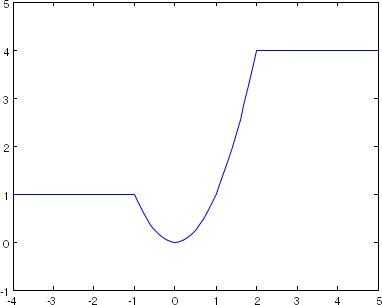
\includegraphics[width=\linewidth]{Pics/forked-function}
\end{columns}
\end{frame}

\begin{frame}[fragile]{Möguleiki: Þrjár if-setningar}
\begin{columns}
\column{0.5\textwidth}
\begin{minted}[frame=lines]{matlab}
if x < -1
    y = 1;
end

if x >= -1 && x <= 2
    y = x^2;
end

if x > 2
    y = 4;
end
\end{minted}
\column{0.5\textwidth}
\begin{itemize}
 \item Virkar, en ekki mjög sniðugt
 \item Ef fyrsta skilyrðið er satt, þá eru hvorug hinna sönn, en þau eru samt reiknuð
 \begin{itemize}
  \item Ekki hagkvæmt
 \end{itemize}
 \item Kóðinn gefur til kynna að öll skilyrðin séu óháð, en þau eru það ekki
\end{itemize}
\end{columns}
\end{frame}

\begin{frame}[fragile]{Möguleiki: Hreiðraðar if-setningar}
\begin{columns}
\column{0.5\textwidth}
\begin{minted}[frame=lines]{matlab}
if x < -1
    y = 1;
else
    if x <= 2
        y = x^2;
    else
        y = 4;
    end
end
\end{minted}
\column{0.5\textwidth}
\begin{itemize}
 \item Notum nýtt trix - \texttt{if} setning inni í \texttt{if} setningu
 \item Vitum að ef $x$ er ekki minna en -1, þá hlýtur það að vera einn af hinum tveimur möguleikunum
 \item Veljum á milli þeirra með seinni \texttt{if}-setningunni
 \item Galli (hér): Kóðinn lítur ekki lengur út eins og skilgreining fallsins
\end{itemize}
\end{columns}
\end{frame}

\begin{frame}[fragile]{Möguleiki: elseif}
\begin{columns}
\column{0.5\textwidth}
\begin{minted}[frame=lines]{matlab}
if x < -1
    y = 1;
elseif x>=-1 && x<=2
    y = x^2;
elseif x > 2
    y = 4;
end
\end{minted}
\column{0.5\textwidth}
\begin{itemize}
 \item Mjög svipað og hreiðraðar if-setningar
 \begin{itemize}
  \item Þetta er er þó læsilegra, sérstaklega ef möguleikarnir eru margir
  \item Hér hefur elseif líka þann kost að líkjast upphaflegri lýsingu á vandamálinu (fallinu)
 \end{itemize}
 \item Möguleikarnir eru metnir hver á fætur öðrum
\end{itemize}
Getum við gert betur?
\end{columns}
\end{frame}

\begin{frame}[fragile]{Möguleiki: elseif}
\begin{columns}
\column{0.5\textwidth}
\begin{minted}[frame=lines]{matlab}
if x < -1
    y = 1;
elseif x <= 2
    y = x^2;
else
    y = 4;
end
\end{minted}
\column{0.5\textwidth}
\begin{itemize}
 \item Óþörf skilyrði hafa hér verið fjarlægð
 \item Niðurstaða er alltaf sú sama, vegna röð samanburðanna
 \item Örlítið skilvirkara, ekki jafn líkt upphaflega vandamálinu
 \begin{itemize}
  \item Er það betra?
 \end{itemize}
\end{itemize}
\end{columns}
\end{frame}

\begin{frame}[fragile]{Annað dæmi um elseif}
\begin{columns}
\column{0.4\textwidth}
Breytt úr talnaeinkunn yfir í stafaeinkunn:
\column{0.6\textwidth}
\begin{minted}[frame=lines]{matlab}
if numGrade == 9 || numGrade == 10
    charGrade = 'A';
elseif numGrade == 8
    charGrade = 'B';
elseif numGrade == 7
    charGrade = 'C';
elseif numGrade == 6
    charGrade = 'D'
else
    charGrade = 'F';
end
\end{minted}
\end{columns}
\end{frame}

\subsection{Switch (4.4)}
\begin{frame}[fragile]{Annar möguleiki: switch}
\begin{columns}
\column{0.4\textwidth}
\begin{itemize}
 \item Oft er hægt að nota \texttt{switch} setningu í stað \texttt{if} setningar með marga \texttt{elseif} hluta
 \begin{itemize}
  \item Þegar mörg tilfelli hafa sömu útkomu má nota slaufusviga til að afmarka
  \item Undir lok \texttt{switch} getur komið \texttt{otherwise} (ekki \texttt{else})
 \end{itemize}

\end{itemize}

\column{0.6\textwidth}
\vspace{\baselineskip}
\begin{minted}[frame=lines]{matlab}
switch numGrade
    case {10, 9}
        charGrade = 'A';
    case 8
        charGrade = 'B';
    case 7
        charGrade = 'C';
    case 6
        charGrade = 'D';
    otherwise
        charGrade = 'F';
end
\end{minted}
\end{columns}
\end{frame}

\begin{frame}{Munur á switch og elseif}
\begin{itemize}
 \item \texttt{switch}-setningin ræður aðeins við að velja á milli einstakra gilda
 \begin{itemize}
  \item Notað fyrir heiltölur eða bókstafi
 \end{itemize}
 \item \texttt{elseif} getur haft almennt skilyrði
 \begin{itemize}
  \item Mun öflugra, en stundum óþarfi
 \end{itemize}
 \item Þegar \texttt{switch} virkar og tilfellin eru ``mörg'' getur hann verið meira viðeigandi en \texttt{elseif}
 \begin{itemize}
  \item Auðlæsilegra?
  \item Hraðvirkara?
 \end{itemize}
\end{itemize}
\end{frame}

\subsection{Try/Catch}

\begin{frame}[fragile]{Try og catch}
\begin{columns}
\column{0.5\textwidth}
\begin{itemize}
 \item Þegar von er á villum við keyrslu kóða má nota sérstaka stýrisetningu, \texttt{try/catch}
 \begin{itemize}
  \item Þá er fyrst \emph{reynt} að framkvæma ákveðnar skipanir
  \item Komi upp villa er hún \emph{gripin} og meðhöndlaðar sérstaklega
 \end{itemize}
\end{itemize}
\column{0.6\textwidth}
Form \texttt{try/catch}:
\begin{verbatim}
try
   "áhættusamar" skipanir
catch
   skipanir sem meðhöndla villu
end
\end{verbatim}
\end{columns}
\end{frame}

\begin{frame}[fragile]{Dæmi um try og catch}
Séu $A$ og $B$ fylki af \emph{óþekktri} stærð getum við haldið útreikningum áfram þó að villa komi upp
\begin{minted}[frame=lines]{matlab}
try
    C= A*B;
catch
    warning('Varúð, C gefið sjálfgefið gildi.');
    C = eye(size(a));
end

\end{minted}
\texttt{warning} virkar eins og \texttt{disp}. Sjá einnig: \texttt{error}.
\end{frame}


\begin{frame}[fragile]{Notkun try og catch}
\begin{itemize}
 \item Hvenær skal nota \texttt{try/catch}?
 \begin{itemize}
  \item Þegar vitað er að ákveðnar, fyrirsjáanlegar villur geta reglulega skotið upp kollinum
  \item Þegar villumeðhöndlun með engu nema \texttt{if} gengur illa
  \begin{itemize}
   \item Notið \texttt{if} þegar það er hægt!
   \item \texttt{try/catch} er fyrir villur, ekki eðlilega keyrslu
  \end{itemize}
 \end{itemize}
 \item Algeng notkunartilvik: Þegar verið er að sækja gögn úr skrá eða af netinu
 \begin{itemize}
  \item Getum treyst eigin kóða, getum ekki treyst umheiminum
 \end{itemize}
\end{itemize}
\end{frame}

\begin{frame}{Meira um try og catch}
\begin{itemize}
 \item \ldots \texttt{try/catch} virðist því miður ekki vera í bókinni
 \begin{itemize}
  \item Engu að síður, mikið notað
 \end{itemize}
 \item Vísa til Matlab-hjálparinnar upp á frekara lesefni:
 \begin{itemize}
  \item \url{http://se.mathworks.com/help/matlab/ref/try.html}
 \end{itemize}
\end{itemize}
\end{frame}

\begin{frame}{Fyrirlestraræfing}
\begin{enumerate}
 \item Skrifið (eina) stýrisetningu sem skrifar 'nótt' ef breytan \texttt{time} er 0 til 6, 'morgunn' fyrir 6 til 12, 'dagur' fyrir 12 til 19 og 'kvöld' fyrir 19 til 24
 \item Skrifið \texttt{try/catch} sem reynir að lesa úr skránni \texttt{ekkiTil.dat} með \texttt{load} skipun. Sé hún ekki til skal þess í stað gera \texttt{ekkiTil} að tómum vigri.
\end{enumerate}
\end{frame}

\section{Gildrur í samanburði}

\begin{frame}{Algengar gildrur í stýriskipunum}
\begin{itemize}
 \item Flestar gildrur í stýriskipunum tengjast skilyrðum \texttt{if}-setningar
 \item Matlab grípur sum mistök
 \begin{itemize}
  \item Gefur villuskilaboð
  \item \textbf{Alltaf að lesa villuskilaboðin!}
  \begin{itemize}
   \item Þau eru stundum gagnleg
   \item Verða gagnlegri eftir því sem innviði Matlab verða kunnuglegri
  \end{itemize}
 \end{itemize}
 \item Erfiðustu villurnar eru þær sem Matlab samþykkir
 \begin{itemize}
  \item Skipunin lögleg, en þýðir ekki það sem við áttum við
  \item Fáum einfaldlega rangar niðurstöður
 \end{itemize}
\end{itemize}
\end{frame}

\begin{frame}{Villur sem Matlab grípur}
\begin{itemize}
 \item Að nota \texttt{=} í stað \texttt{==} til að athuga hvort gildi séu jöfn
 \begin{itemize}
  \item \texttt{if fjoldi = 0}
  \begin{itemize}
   \item {\color{red} Error: The expression to the left of the equals sign is not a valid target for an assignment.}
  \end{itemize}
 \end{itemize}
 \item Að gleyma gæsalöppum
 \begin{itemize}
 \item \texttt{if letter == y}
  \begin{itemize}
   \item {\color{red} ??? Undefined function or variable 'y'.}
   \item \ldots nema að \texttt{y} sé fyrir tilviljun skilgreind breyta, þá kemur engin villa
  \end{itemize}
 \end{itemize}
\end{itemize}
\end{frame}

\begin{frame}{Villur sem Matlab grípur ekki}
\begin{itemize}
 \item Dæmi: Tvöfaldur samanburður
 \begin{itemize}
  \item \texttt{if 0 < x < 5}
  \begin{itemize}
   \item Þetta skilyrði er alltaf satt, sama hvaða gildi x hefur
   \item Fyrst reiknað $(0 < x)$, sem gefur $0$ eða $1$.  Bæði $0$ og $1$ eru minni en $5$!
  \end{itemize}
 \end{itemize}
 \item Ætluðum (líklega) að skrifa:
 \begin{itemize}
 \item \texttt{if (0 < x) \&\& (x < 5)}
  \begin{itemize}
   \item Satt þegar \texttt{x} er á milli $0$ og $5$
  \end{itemize}
 \end{itemize}
\end{itemize}
\end{frame}

\begin{frame}{Villur sem Matlab grípur ekki}
\begin{itemize}
 \item Enn erfiðara dæmi - villur sem stundum koma upp
 \begin{itemize}
  \item \texttt{if lengd || haed <= 0}
  \begin{itemize}
   \item Þetta skilyrði er satt ef \texttt{lengd} er ekki 0 eða ef \texttt{haed} er neikvæð tala
  \end{itemize}
 \end{itemize}
 \item Ætluðum (líklega) að skrifa:
 \begin{itemize}
 \item \texttt{if lengd <= 0 || haed <= 0}
  \begin{itemize}
   \item Satt þegar önnur hvor breytan er ekki jákvæð
  \end{itemize}
 \end{itemize}
\end{itemize}
\end{frame}


\section{is-föll (4.6)}

\begin{frame}{is-Föll í Matlab}
\begin{itemize}
 \item Mörg föll í Matlab til að athuga hvort einhver eiginleiki gildi
 \begin{itemize}
  \item Þau skila sanngildi (satt/ósatt)
  \item Langflest þeirra byrja á enska orðinu ``is''
  \item Notuð til að athuga ýmislegt, t.d.
  \begin{itemize}
   \item tegund breytu (heiltala, kommutala, bókstafur, \ldots)
   \item gerð breytu (tala, vigur, fylki)
  \end{itemize}
 \end{itemize}
\end{itemize}
\end{frame}

\begin{frame}[fragile]{Dæmi: isletter fallið}
\begin{columns}
\column{0.35\textwidth}
\begin{itemize}
 \item \texttt{isletter} skilar \emph{satt} ef inntakið er bókstafur
 \begin{itemize}
  \item Þ.e. ekki tölustafur, greinarmerki eða sértákn
  \item Ræður við íslenska stafi
  \item Skilar \emph{ósatt} sé inntak ekki af taginu char
 \end{itemize}
\end{itemize}
\column{0.65\textwidth}
\begin{minted}[frame=lines]{matlab}
symb = input('Sláðu inn staf: ','s');
if isletter(symb)
    disp('Þetta er bókstafur');
else
    disp('Þetta er ekki bókstafur');
end
\end{minted}
\end{columns}
\end{frame}

\begin{frame}[fragile]{Dæmi: isempty fallið}
\begin{columns}
\column{0.3\textwidth}
\begin{itemize}
 \item \texttt{isempty} skilar \emph{satt} sé breyta tóm
 \begin{itemize}
  \item \emph{Ósatt} innihaldi breytan gildi
 \end{itemize}
 \item breytan þarf þó að vera skilgreind
\end{itemize}
\column{0.7\textwidth}
\begin{minted}[frame=lines]{matlab}
>> format compact
>> v = [];
>> isempty(v)
ans =  1
>> v = [1, 2];
>> isempty(v)
ans = 0
>> clear
>> isempty(v)
??? Undefined function or variable 'v'.
\end{minted}
\end{columns}
\end{frame}

\begin{frame}[fragile]{Dæmi: exist fallið}
\begin{columns}
\column{0.5\textwidth}
\begin{itemize}
 \item Hægt að athuga hvort breyta, fall eða annað sé skilgreint með fallinu \texttt{exist}
 \item Tekur inn nafn í streng
 \begin{itemize}
  \item Skilar 0 sé nafnið ekki skilgreint
  \item Aðrar tölur eftir gerð fyrirbrigðisins sem nafnið vísar til
 \end{itemize}
\end{itemize}
\column{0.5\textwidth}
\begin{minted}[frame=lines]{matlab}
>> x = 1;
>> exist('x')
ans =  1
>> exist('sin')
ans =  5
>> exist('y')
ans = 0
\end{minted}
\end{columns}
\end{frame}

\begin{frame}{Fleiri is-föll}
\begin{center}
\begin{tabular}{ll}
\toprule
Fall&Spurning\\
\midrule
\texttt{isnumeric}&Er inntakið tala?\\
\texttt{isinteger}&Er inntakið af heiltölutagi?\\
\texttt{iscolumn}&Er inntakið dálkvigur?\\
\texttt{isrow}&Er inntakið línuvigur?\\
\texttt{issorted}&Er inntakið raðaður vigur?\\
\texttt{isvarname}&Er inntakið strengur með löglegu breytunafni?\\
\bottomrule
\end{tabular}
\end{center}
\end{frame}

\section{Lykkjuhugtakið}

\begin{frame}{Hugtakið ``lykkja''}
\begin{itemize}
 \item Hingað til hefur hver skipun verið framkvæmd nákvæmlega einu sinni
 \item Við getum látið Matlab endurtaka framkvæmd skipunar, oftast með smávægilegum breytingum, með því að nota lykkju (e. \emph{loop})
 \begin{itemize}
  \item Kynnumst lykkjum í næstu viku
 \end{itemize}

%  \item Þegar röð skipana er keyrð inni í lykkju ``hoppar'' Matlab aftur upp í byrjun raðarinnar þegar röðinni er lokið, þar til ákveðnu skilyrði er náð.
\end{itemize}
\end{frame}


\begin{frame}[fragile]{Fyrirlestraræfing}
\begin{columns}
\column{0.5\textwidth}
\begin{enumerate}
\setcounter{enumi}{2}
 \item Hver eru lokagildi breytanna \texttt{a} og \texttt{b} í forritsbútnum hér til hliðar?
 \item Skrifið ykkar eigin útgáfu af \texttt{isrow} fallinu. Nota má innbyggð föll önnur en \texttt{isrow} sjálft. (Ráðlegging: notið \texttt{size} fallið)
\end{enumerate}
\column{0.5\textwidth}
\begin{minted}[frame=lines]{matlab}
a = 2; 
b = 5;
if a < b
   a = b; 
   b = a;
end
if a > b
   a = 2;
end
\end{minted}
\end{columns}
\end{frame}

\end{document}
